
%%%%%%%%%%%%%%%%%%%%%%%%%%%%%%%%%%%%%%%%%%%%%%%%%%%%%%%%%%%%%%%%%%%%%%
%%                     Necessary_Stim
%%%%%%%%%%%%%%%%%%%%%%%%%%%%%%%%%%%%%%%%%%%%%%%%%%%%%%%%%%%%%%%%%%%%%%

\subsection{Glyph: \glyph{Necessary stimulation}}\label{sec:necessary_stim}

A necessary stimulation, is one that is necessary for a process to take place. A process modulated by a necessary stimulation can only occur when this necessary stimulation is active. The target extremity of a \glyph{necessary stimulation} carries an open arrow (to remind that it is a \glyph{stimulation}) coming after a larger vertical bar.

\begin{figure}[H]
  \centering
  
\includegraphics[scale = 0.5]{images/necessary_stim}
  \caption{The \PD glyph for \glyph{Necessary Stimulation}.}
  \label{fig:Necessary Stimulation}
\end{figure}

The example in \fig{necessary_stim-gene} below describes the transcription of a gene~X, that is the creation of a messenger RNA~X triggered by the gene~X.  The creation of the protein~X is then triggered by the mRNA~X.  (Note that the same example could be represented using the gene as reactant and product, although it is semantically different.)

\begin{figure}[H]
  \centering
  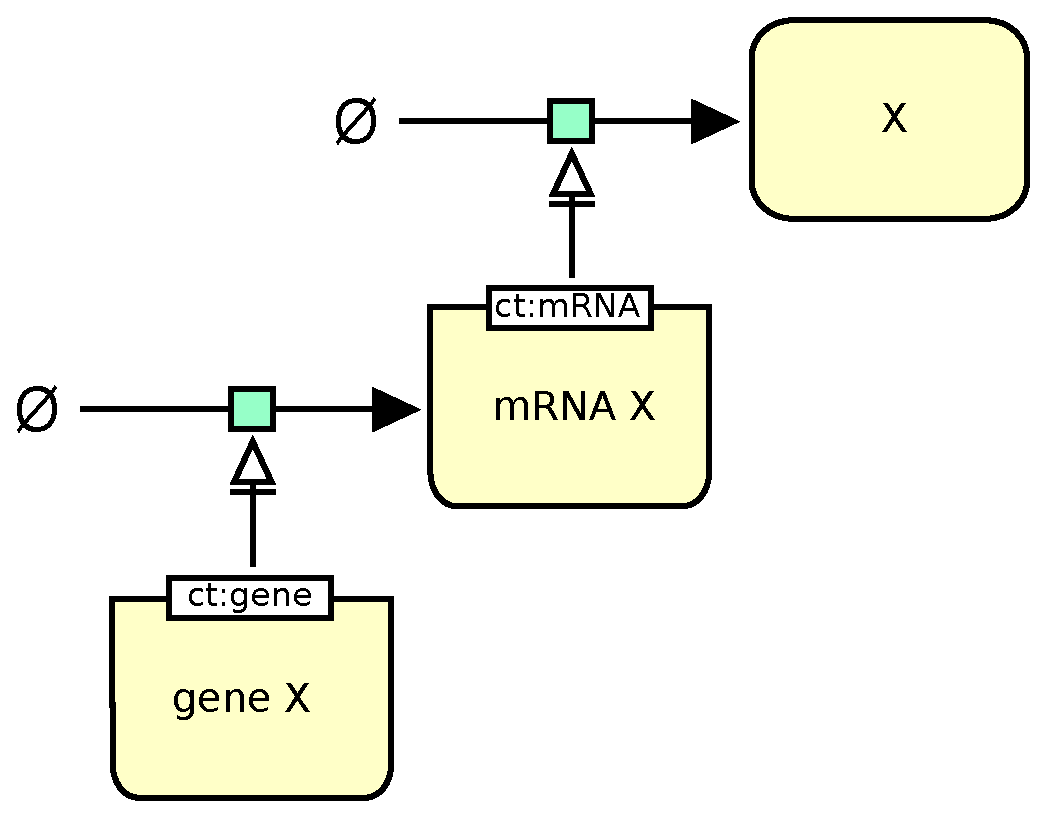
\includegraphics[scale = 0.5]{images/necessary_stim-genetic}
  \caption{The creation of a messenger RNA~X triggered by the gene~X.}
  \label{fig:necessary_stim-gene}
\end{figure}


The example in \fig{necessary_stim-calcium} below describes the transport of calcium ions out of the endoplasmic reticulum. Without IP3 receptor, there is not calcium flux, therefore, one cannot use a \glyph{stimulation}. The Necessary Stimulation instead represents this absolute stimulation.

\begin{figure}[H]
  \centering
  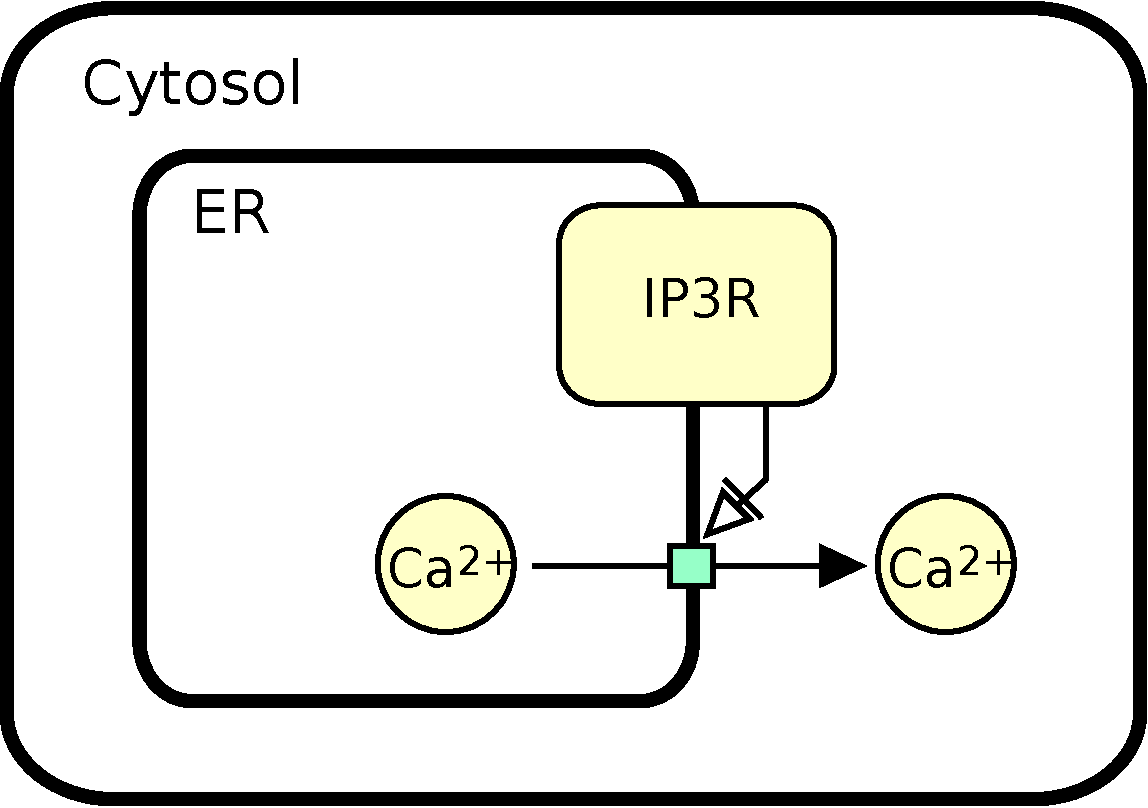
\includegraphics[scale = 0.5]{images/necessary_stim-transport}
  \caption{The transport of calcium ions out of the endoplasmic reticulum into the cytosol. Note that IP3R crosses both compartment boundaries. This is allowed, but the Macromolecule should only belong to one of the compartments.}
  \label{fig:necessary_stim-calcium}
\end{figure}
